%!TEX program = pdflatex
\documentclass[UTF8]{article}

\usepackage[UTF8]{ctex}
\usepackage{amsmath}
\usepackage{enumerate}
\usepackage{amssymb}
\usepackage{graphicx}
\usepackage{booktabs}
 
\title{Homework 11.02}
\date{}
    \begin{document}
    \maketitle
    \section{Question 39}
    \paragraph{Question}
    Determine the number of solutions of the equation $ x_{1} + x_{2} + x_{3} + x_{4} = 14 $ in nonnegative integers $ x_{1} $, $ x_{2} $, $ x_{3} $, and $ x_{4} $ not exceeding 8.
    \paragraph{Answer}
    \begin{center}
        For $ 1 \leq i \leq 4 $ let $ A_{i} $ denote the set of elements in $S$ with $x_{i} \geq 9$. \\
        We seek $\vert \bar{A_{1}} \cap \bar{A_{2}} \cap \bar{A_{3}} \cap \bar{A_{4}}\vert. $ \\
        \vspace{6pt}
        \begin{tabular}{c|c|c}
            \toprule
            set & size & justification\\
            \midrule
            $S$ & $\begin{pmatrix} 17 \\ 3 \end{pmatrix}$ & $17 = 14 + 4 - 1$\\
            $A_{i}$ & $\begin{pmatrix} 8 \\ 3 \end{pmatrix}$ & $17 - 9 = 8$\\
            $A_{i} \cap A_{j}$ & $ 0 $ & $17 - 9 - 9 = -1 < 3$\\
            \bottomrule
        \end{tabular} \\
        By inclusion/exclusion \\
        $\vert \bar{A_{1}} \cap \bar{A_{2}} \cap \bar{A_{3}} \cap \bar{A_{4}}\vert. $ = $\begin{pmatrix} 17 \\ 3 \end{pmatrix} - 4\begin{pmatrix} 8 \\ 3 \end{pmatrix} = 456$
    \end{center}
    \section{Question 40}
    \paragraph{Question}
    At a party seven gentlemen check their hats. In how many ways can their hats be returned so that
    \begin{enumerate}[(a)]
    \item no gentleman receives his own hat?
    \item at least one of the gentlemen receives his own hat?
    \item at least two of the gentlemen receive their own hats?
    \end{enumerate}
    \paragraph{Answer}
    \begin{center}
        \begin{enumerate}[(a)]
            \item $D_{7} = 1854$
            \item $7! - D_{7} = 3186$
            \item Let $A_{i}$ be the set of all permutations of the set ${1, 2, . . . , n}$ having exactly $i$ numbers in their own natural positions. \\
                  Then $ \vert A_{i} \vert = \begin{pmatrix} n \\ i \end{pmatrix}D_{n - i}$ \\
                  Then $ A_{0} \cup A_{1} $ is the set of all permutations with at most 1 number in its natural position. \\
                  Then $ \vert A_{0} \cup A_{1} \vert = \vert A_{0} \vert + \vert A_{1} \vert = D_{n} + \begin{pmatrix} n \\ 1 \end{pmatrix}D_{n - 1}$ \\
                  Thus the answer to (c) is $ 7! - D_{7} - 7D_{6} = 1331 $.
        \end{enumerate}
    \end{center}

    \section{Question 41}
    \paragraph{Question}
    What is the number of ways to place six nonattacking rooks on the 6-by-6 boards with forbidden positions as shown?
    \begin{figure}[ht]
        \centering
        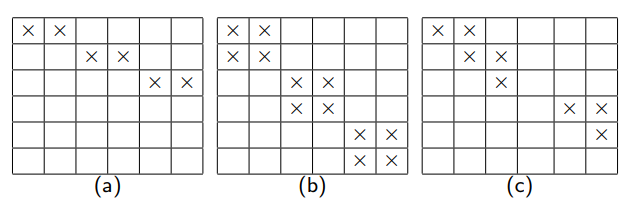
\includegraphics[scale=0.6]{img/t41.png}
        \end{figure}
    
    \paragraph{Answer}
    \begin{center}
        $$ R_{n}(C) = \sum_{k = 0}^{n}{(-1)}^{k}r_{k}(C){(n - k)}! $$
        \begin{enumerate}[(a)]
            \item  Since $ r_{0} = 1 $,$ r_{1} = 6 $,$ r_{2} = 3 × 2 × 2 = 12 $,$ r_{3} = 2 × 2 × 2 = 8 $,$ r_{4} = r5 = r6 = 0 $, then \\
                $ R_{6}(C) = 6! − 6 × 5! + 12 × 4! − 8 × 3! $
            \item Since the rook polynomial \\
                $$ R(C,x) = (1 + 4x + 2x^{2})^{3} $$
                then $r_{0} = 1, r_{1} = 12, r_{2} = 54, r_{3} = 102, r_{4} = 44, r_{5} = 48$, and $r_{6} = 8$. Thus \\
                $ R_{6}(C) = 6! − 12 × 5! + 54 × 4! − 102 × 3! + 44 × 2! − 48 × 1! + 8 × 0! $.
            \item Since the rook polynomial \\
                $$ R(C,x) = (1 + 5x + 6x^{2} + x^{3})(1 + 3x + x^{2})$$
                then $r_{0} = 1, r_{1} = 8, r_{2} = 22, r_{3} = 24, r_{4} = 9, r_{5} = 1$, and $r_{6} = 0$. Thus \\
                $R_{6}(C) = 6! − 8 × 5! + 22 × 4! − 24 × 3! + 9 × 2! − 1!$.
        \end{enumerate}
    \end{center}

    \section{Question 42}
    \paragraph{Question}
    A carousel has eight seats, each representing a different animal. Eight girls are seated on the carousel facing forward (each girl looks at another girl’s back). In how many ways can they change seats so that each has a different girl in front of her? How does the problem change if all the seats are identical?
    \paragraph{Answer}
    \begin{center}
        \begin{figure}[ht]
            \centering
            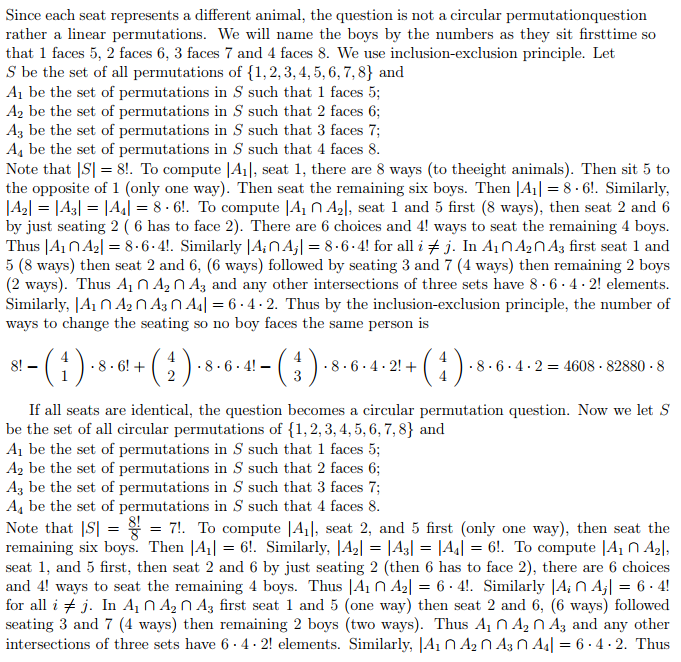
\includegraphics[scale=0.6]{img/t42_a1.png}
            \end{figure}
            \begin{figure}[ht]
                \centering
                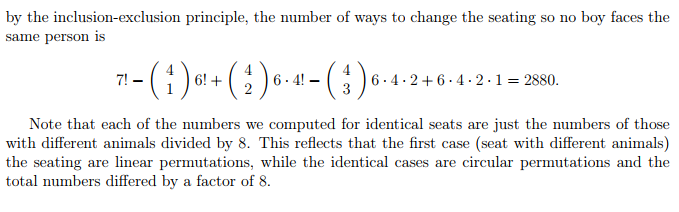
\includegraphics[scale=0.6]{img/t42_a2.png}
                \end{figure}
    \end{center}

    \section{Question 44}
    \paragraph{Question}
    Prove the following about the Fibonacci numbers,
    \begin{enumerate}[(a)]
        \item $ f_{n} $ is even if and only if n is divisible by 3.
        \item $ f_{n} $ is divisible by 3 if and only if n is divisible by 4.
        \item $ f_{n} $ is divisible by 4 if and only if n is divisible by 6.
    \end{enumerate}
    \paragraph{Answer}
    \begin{center}
        \begin{figure}[ht]
            \centering
            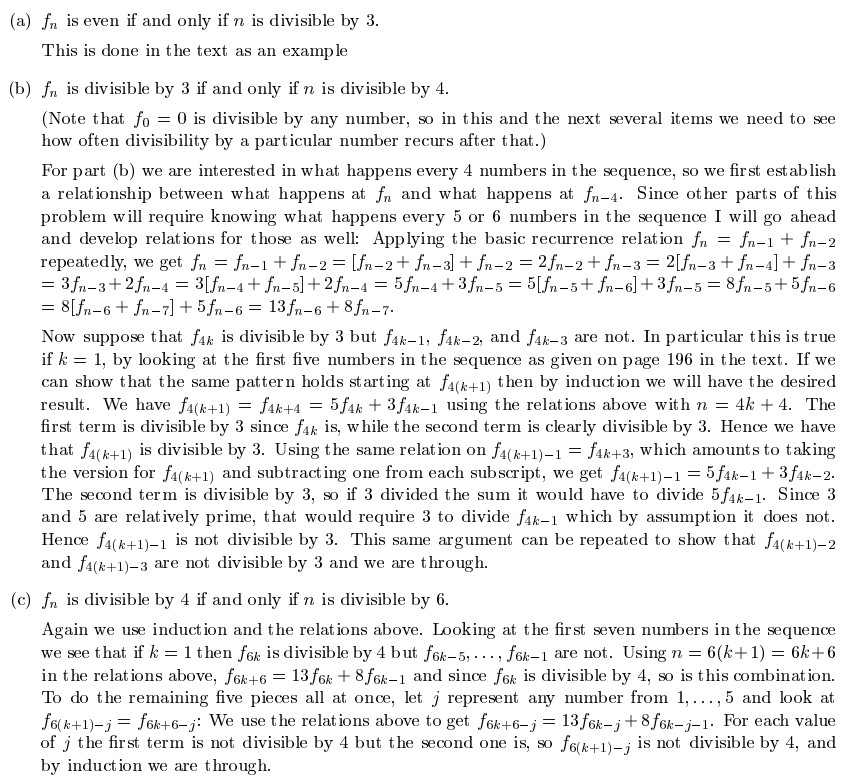
\includegraphics[scale=0.6]{img/t44_a.png}
            \end{figure}
    \end{center}
    \end{document}